\documentclass[11pt,letterpaper]{article}

\usepackage[utf8]{inputenc}
\usepackage[T1]{fontenc}
\usepackage{lmodern}
\usepackage[spanish]{babel}
\usepackage[margin=2.5cm]{geometry}
\usepackage{graphicx}
\usepackage{xcolor}
\usepackage{listings}
\usepackage{fancyhdr}
\usepackage{hyperref}

\hypersetup{colorlinks=true, urlcolor=blue}

\pagestyle{fancy}
\fancyhf{}
\fancyhead[L]{ICN-292 --- Sistemas de Información para la Gestión}
\fancyhead[R]{Laboratorio 5 | 2026-2}
\fancyfoot[C]{\thepage}

\lstset{
    language=SQL,
    basicstyle=\ttfamily\small,
    keywordstyle=\color{blue}\bfseries,
    stringstyle=\color{orange!80!black},
    commentstyle=\color{gray},
    morekeywords={LIMIT, BETWEEN, ENUM, AUTO_INCREMENT, IF, EXISTS},
    frame=single,
    breaklines=true,
    columns=fullflexible,
    keepspaces=true,
    showstringspaces=false,
    literate={á}{{\'a}}1 {é}{{\'e}}1 {í}{{\'i}}1 {ó}{{\'o}}1 {ú}{{\'u}}1
             {Á}{{\'A}}1 {ñ}{{\~n}}1
}

\begin{document}

% ------------------------------------------------------------
% Portada
% ------------------------------------------------------------
\begin{titlepage}
    \centering
    
\includegraphics[width=0.22\textwidth]{img/logo_usm.png}\par
    \vspace{0.8cm}
    {\large\textsc{Universidad Técnica Federico Santa María}\par}
    \vspace{0.2cm}
    ICN-292 --- Sistemas de Información para la Gestión \quad $|$ \quad Semestre 2026-2\par
    \vspace{3cm}
    \rule{0.75\textwidth}{0.6pt}\par
    \vspace{0.6cm}
    {\LARGE\textbf{Laboratorio 5}\par}
    \vspace{0.3cm}
    Consultas SQL sobre la base de Andes Bike\par
    \vspace{0.6cm}
    \rule{0.75\textwidth}{0.6pt}\par
    \vfill
    \raggedright
    \textbf{Alumno:} Claudio Vera Ávila\par\vspace{0.2cm}
    \textbf{Rol:} 202104575-9\par\vspace{0.2cm}
    \textbf{Paralelo:} 100\par\vspace{0.2cm}
    \textbf{Fecha de entrega:} 15 de noviembre de 2026\par\vspace{0.2cm}
    \textbf{Repositorio:} \url{https://github.com/claudioveravila/ICN292-Lab5-Vera-Claudio}\par
    \vspace{1cm}
\end{titlepage}

% ------------------------------------------------------------
% Consultas
% ------------------------------------------------------------
\clearpage
\noindent\begin{minipage}{\linewidth}
\section*{Consulta 1}

Liste todos los vendedores con la cantidad de ventas que registraron, incluidos los que no registraron ninguna. Ordene de mayor a menor cantidad y, a igualdad, por nombre. Los que no tienen ventas deben mostrar cero, no quedar en blanco.

\begin{lstlisting}
SELECT   v.nombre, COUNT(ve.id_venta) AS cantidad_ventas
FROM     vendedores v
LEFT JOIN ventas ve ON v.id_vendedor = ve.id_vendedor
GROUP BY v.id_vendedor, v.nombre
ORDER BY cantidad_ventas DESC, v.nombre;
\end{lstlisting}

\begin{center}
    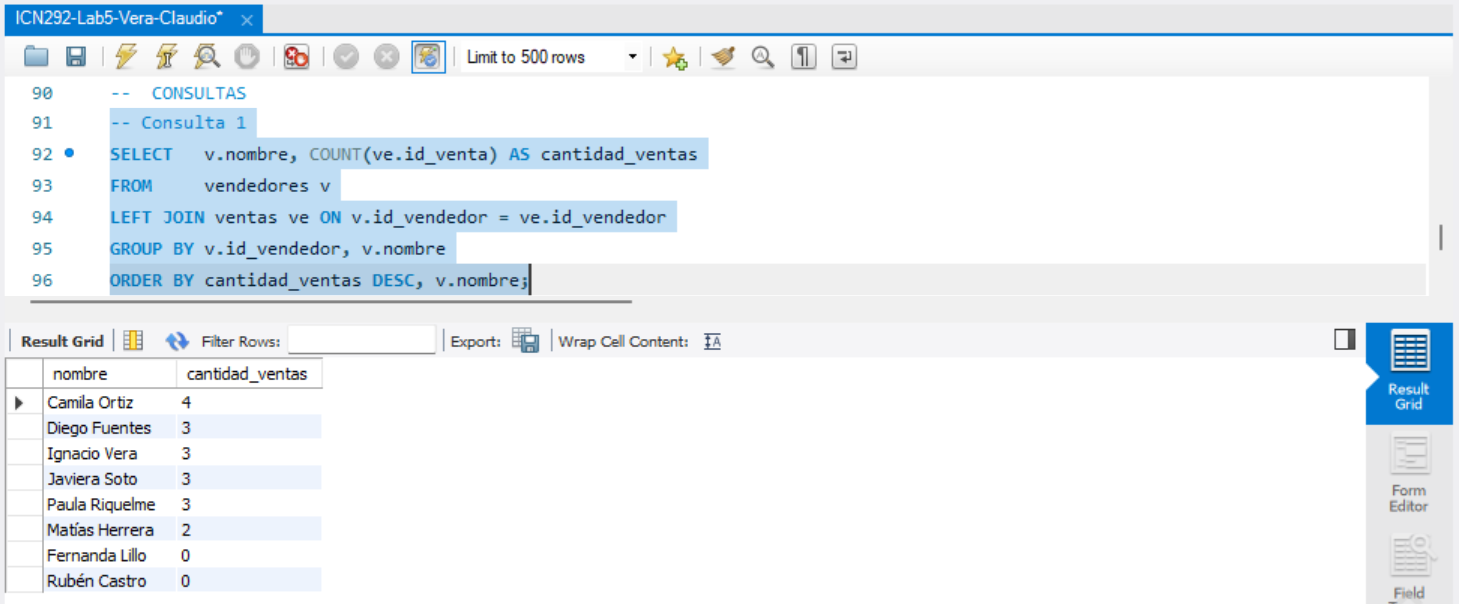
\includegraphics[width=0.72\linewidth]{img/c1.png}
\end{center}
\end{minipage}
\par\vspace{0.6cm}

\noindent\begin{minipage}{\linewidth}
\section*{Consulta 2}

Para cada tienda muestre su nombre, cuántas ventas se registraron y cuántas unidades se vendieron, incluidas las tiendas que no tienen ningún vendedor. Ordene por unidades de mayor a menor.

\begin{lstlisting}
SELECT   t.nombre AS tienda,
         COUNT(ve.id_venta) AS cantidad_ventas,
         SUM(ve.unidades)   AS unidades
FROM     tiendas t
LEFT JOIN vendedores v ON t.id_tienda   = v.id_tienda
LEFT JOIN ventas    ve ON v.id_vendedor = ve.id_vendedor
GROUP BY t.id_tienda, t.nombre
ORDER BY unidades DESC;
\end{lstlisting}

\begin{center}
    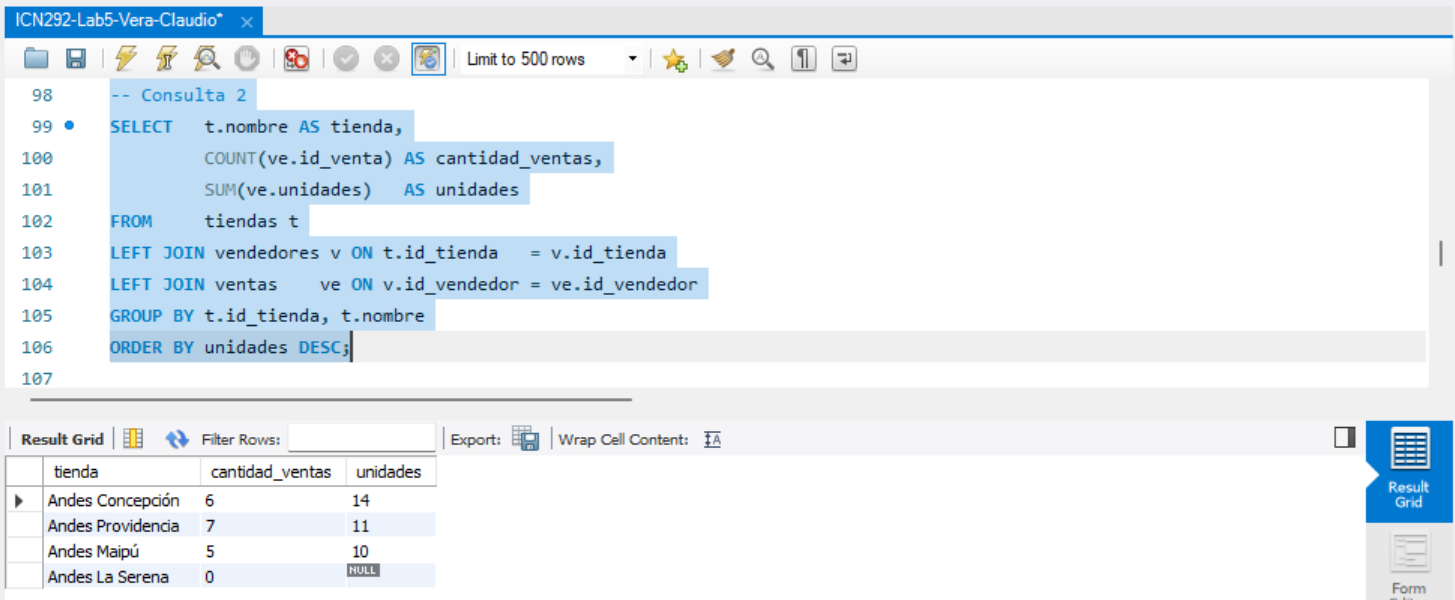
\includegraphics[width=0.72\linewidth]{img/c2.png}
\end{center}
\end{minipage}
\par\vspace{0.6cm}

\noindent\begin{minipage}{\linewidth}
\section*{Consulta 3}

Liste las tiendas que no tienen ningún vendedor asignado.

\begin{lstlisting}
SELECT t.nombre
FROM   tiendas t
LEFT JOIN vendedores v ON t.id_tienda = v.id_tienda
WHERE  v.id_vendedor IS NULL;
\end{lstlisting}

\begin{center}
    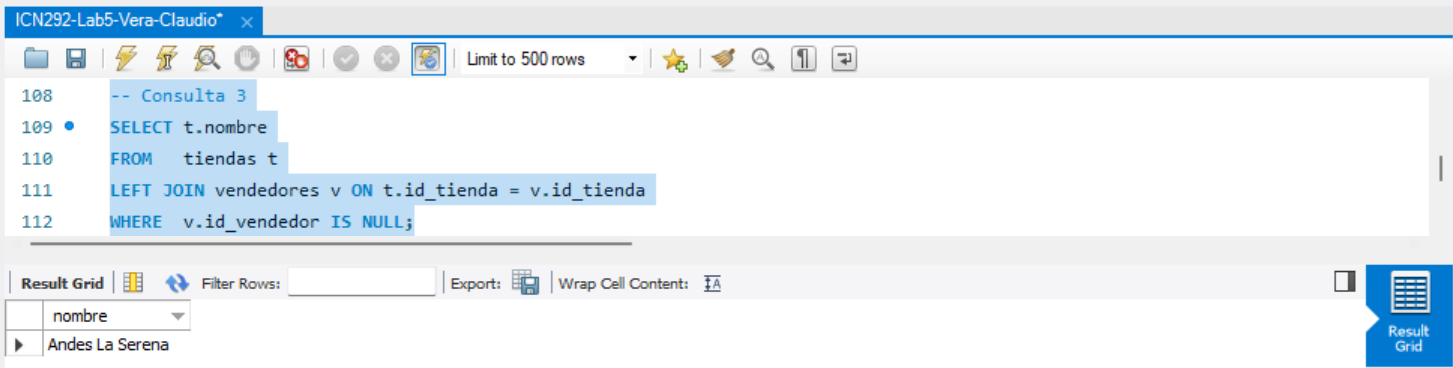
\includegraphics[width=0.72\linewidth]{img/c3.png}
\end{center}
\end{minipage}
\par\vspace{0.6cm}

\noindent\begin{minipage}{\linewidth}
\section*{Consulta 4}

Liste los modelos que no se vendieron ni una sola vez en junio de 2025. Explique en una línea en qué parte de la consulta puso la condición del mes y qué habría devuelto si la hubiera puesto en la otra.

\begin{lstlisting}
SELECT b.modelo
FROM   bicicletas b
LEFT JOIN ventas ve ON b.id_bicicleta = ve.id_bicicleta
                   AND ve.fecha BETWEEN '2025-06-01' AND '2025-06-30'
WHERE  ve.id_venta IS NULL;
\end{lstlisting}

\begin{center}
    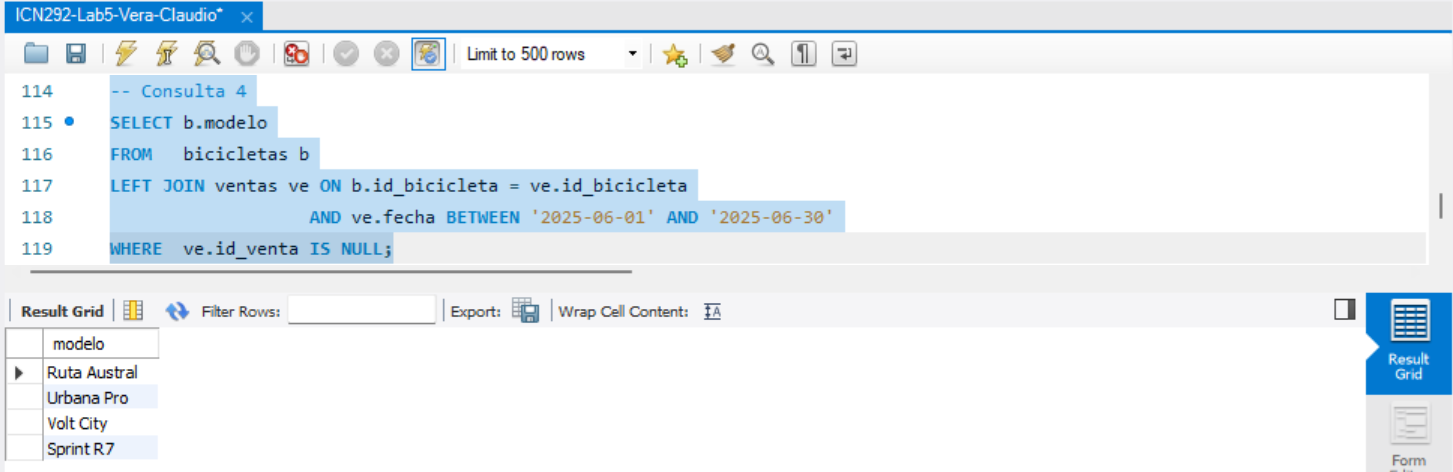
\includegraphics[width=0.72\linewidth]{img/c4.png}
\end{center}

La condición de junio la puse en el \texttt{ON} del \texttt{LEFT JOIN}, para que solo se junten las ventas de ese mes y los que no tuvieron ninguna queden en NULL. Si la condición la colocaba en el \texttt{WHERE}, se filtraba después de unir las tablas y no salía nada.
\end{minipage}
\par\vspace{0.6cm}

\noindent\begin{minipage}{\linewidth}
\section*{Consulta 5}

Liste los vendedores que no han registrado ninguna venta, mostrando también el nombre de su tienda. Ninguno de ellos puede quedar fuera del resultado.

\begin{lstlisting}
SELECT v.nombre, t.nombre AS tienda
FROM   vendedores v
LEFT JOIN ventas  ve ON v.id_vendedor = ve.id_vendedor
LEFT JOIN tiendas t  ON v.id_tienda   = t.id_tienda
WHERE  ve.id_venta IS NULL;
\end{lstlisting}

\begin{center}
    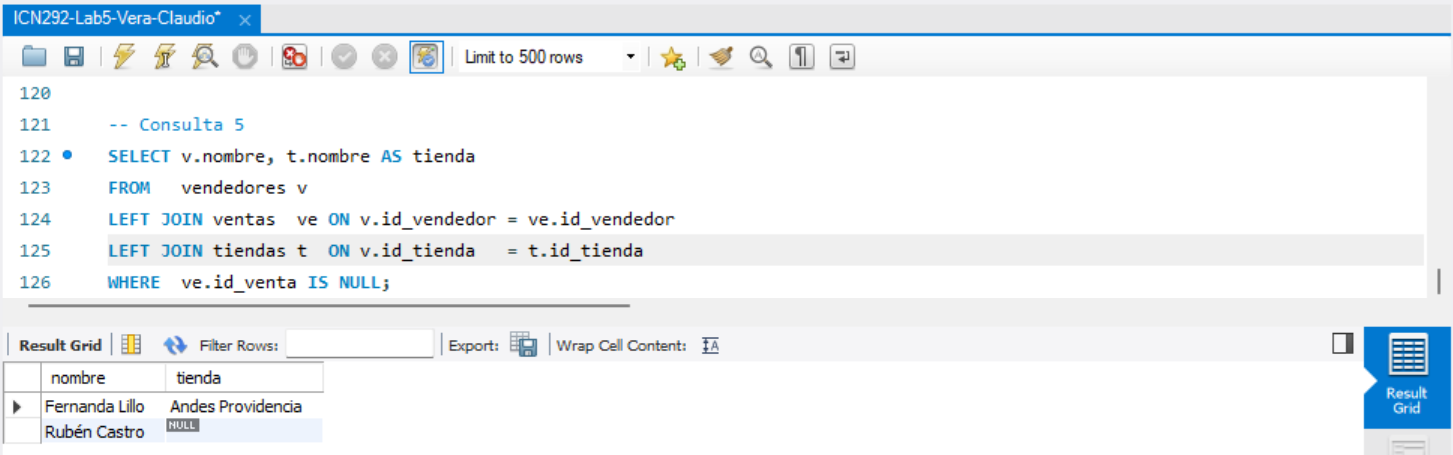
\includegraphics[width=0.72\linewidth]{img/c5.png}
\end{center}
\end{minipage}
\par\vspace{0.6cm}

\noindent\begin{minipage}{\linewidth}
\section*{Consulta 6}

Liste los pares de vendedores que trabajan en la misma tienda, poniendo primero al que ingresó antes. Muestre los dos nombres, las dos fechas de ingreso y la tienda. Cada par debe aparecer una sola vez.

\begin{lstlisting}
SELECT v1.nombre        AS vendedor_1,
       v1.fecha_ingreso AS ingreso_1,
       v2.nombre        AS vendedor_2,
       v2.fecha_ingreso AS ingreso_2,
       t.nombre         AS tienda
FROM   vendedores v1
JOIN   vendedores v2 ON v1.id_tienda     = v2.id_tienda
                    AND v1.fecha_ingreso < v2.fecha_ingreso
JOIN   tiendas t     ON v1.id_tienda     = t.id_tienda
ORDER BY t.nombre, v1.fecha_ingreso;
\end{lstlisting}

\begin{center}
    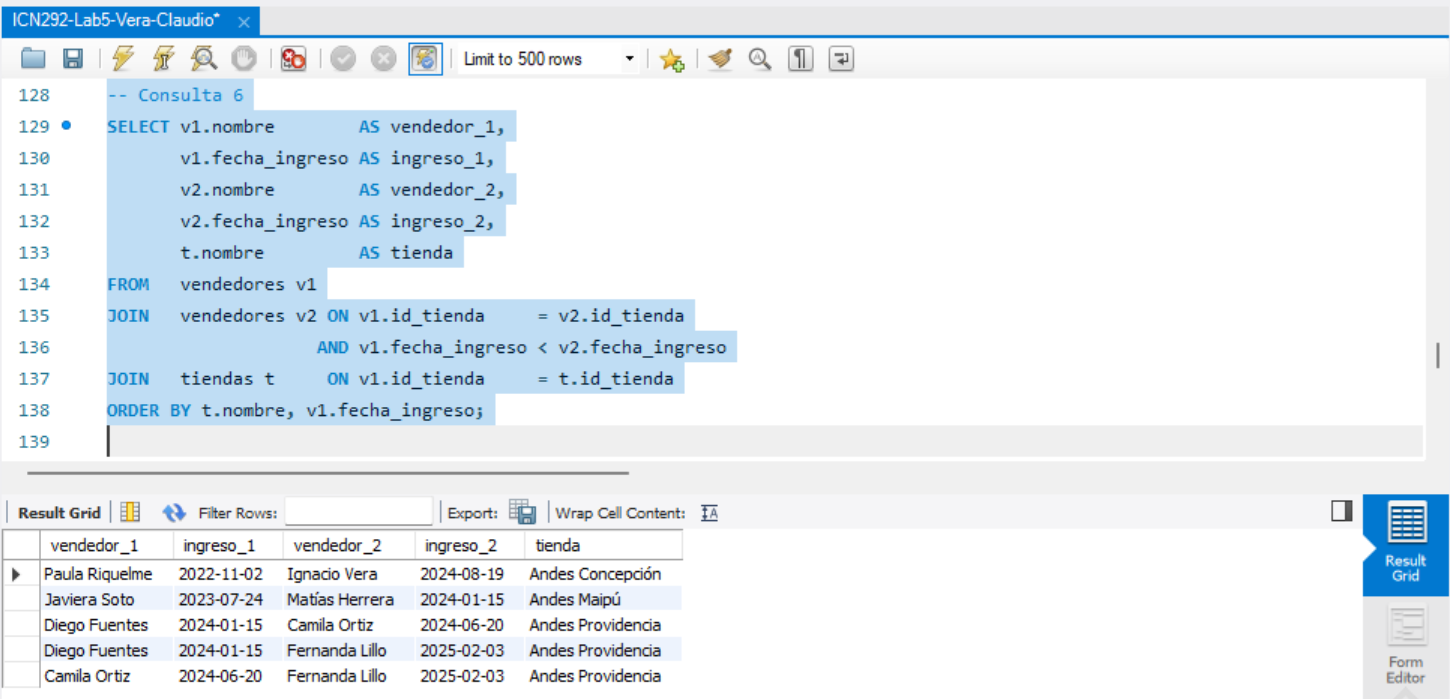
\includegraphics[width=0.72\linewidth]{img/c6.png}
\end{center}
\end{minipage}
\par\vspace{0.6cm}

\noindent\begin{minipage}{\linewidth}
\section*{Consulta 7}

Para cada tienda, calcule el monto total vendido en bicicletas de las categorías `Montaña' y `Ruta', dejando solo las tiendas que superan los 2.000.000. Ordene de mayor a menor.

\begin{lstlisting}
SELECT   t.nombre AS tienda,
         SUM(ve.unidades * b.precio) AS monto_total
FROM     tiendas t
JOIN     vendedores v  ON t.id_tienda    = v.id_tienda
JOIN     ventas     ve ON v.id_vendedor  = ve.id_vendedor
JOIN     bicicletas b  ON ve.id_bicicleta = b.id_bicicleta
WHERE    b.categoria IN ('Montaña', 'Ruta')
GROUP BY t.id_tienda, t.nombre
HAVING   SUM(ve.unidades * b.precio) > 2000000
ORDER BY monto_total DESC;
\end{lstlisting}

\begin{center}
    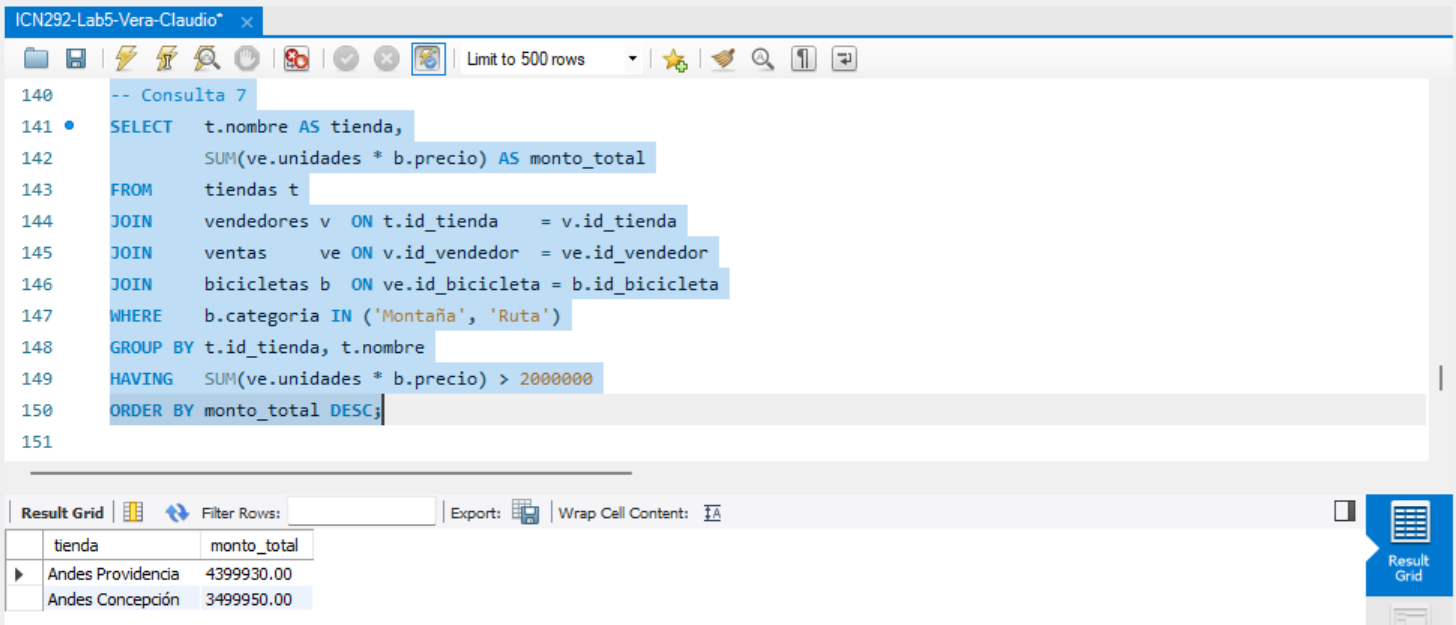
\includegraphics[width=0.72\linewidth]{img/c7.png}
\end{center}
\end{minipage}
\par\vspace{0.6cm}

\noindent\begin{minipage}{\linewidth}
\section*{Consulta 8}

Liste el modelo y el precio de las bicicletas cuyo precio supera el promedio del catálogo, de mayor a menor. Indique en el informe el valor de ese promedio y de dónde lo obtuvo.

\begin{lstlisting}
SELECT   modelo, precio
FROM     bicicletas
WHERE    precio > (SELECT AVG(precio)
                   FROM bicicletas)
ORDER BY precio DESC;
\end{lstlisting}

\begin{center}
    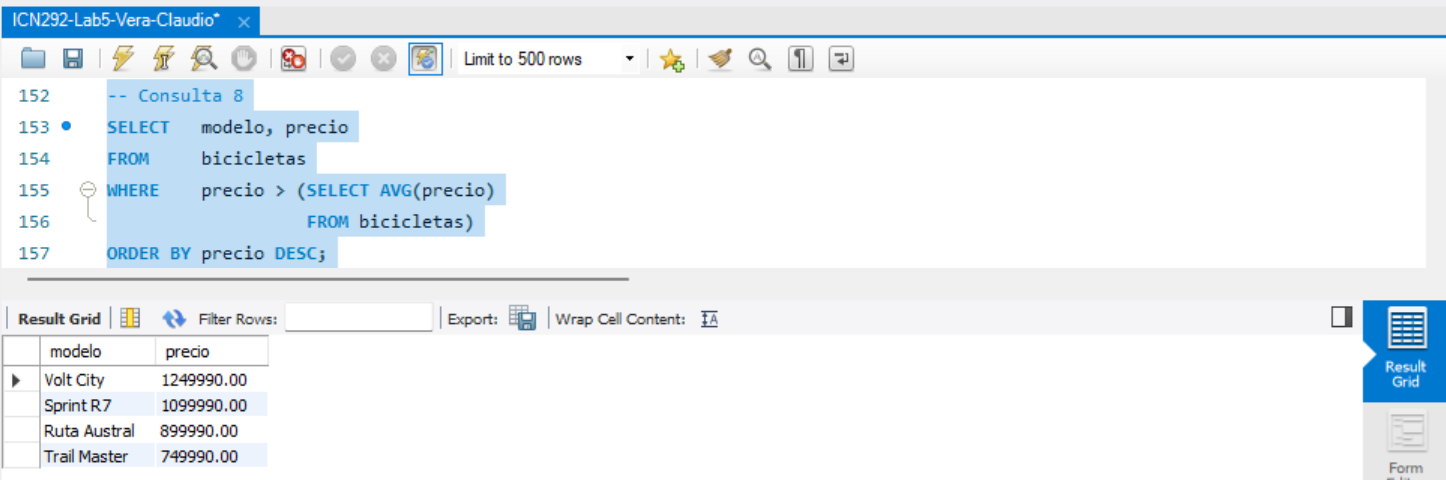
\includegraphics[width=0.72\linewidth]{img/c8.png}
\end{center}

El promedio es 657.490 y lo saqué de la subconsulta \texttt{SELECT AVG(precio) FROM bicicletas}, que promedia el precio de los 8 modelos.
\end{minipage}
\par\vspace{0.6cm}

\noindent\begin{minipage}{\linewidth}
\section*{Consulta 9}

Liste los vendedores cuyo promedio de unidades por venta supera el promedio de unidades de todas las ventas de la cadena. Muestre el nombre y su promedio, de mayor a menor y, a igualdad, por nombre.

\begin{lstlisting}
SELECT   v.nombre, AVG(ve.unidades) AS promedio_unidades
FROM     vendedores v
JOIN     ventas ve ON v.id_vendedor = ve.id_vendedor
GROUP BY v.id_vendedor, v.nombre
HAVING   AVG(ve.unidades) > (SELECT AVG(unidades)
                             FROM ventas)
ORDER BY promedio_unidades DESC, v.nombre;
\end{lstlisting}

\begin{center}
    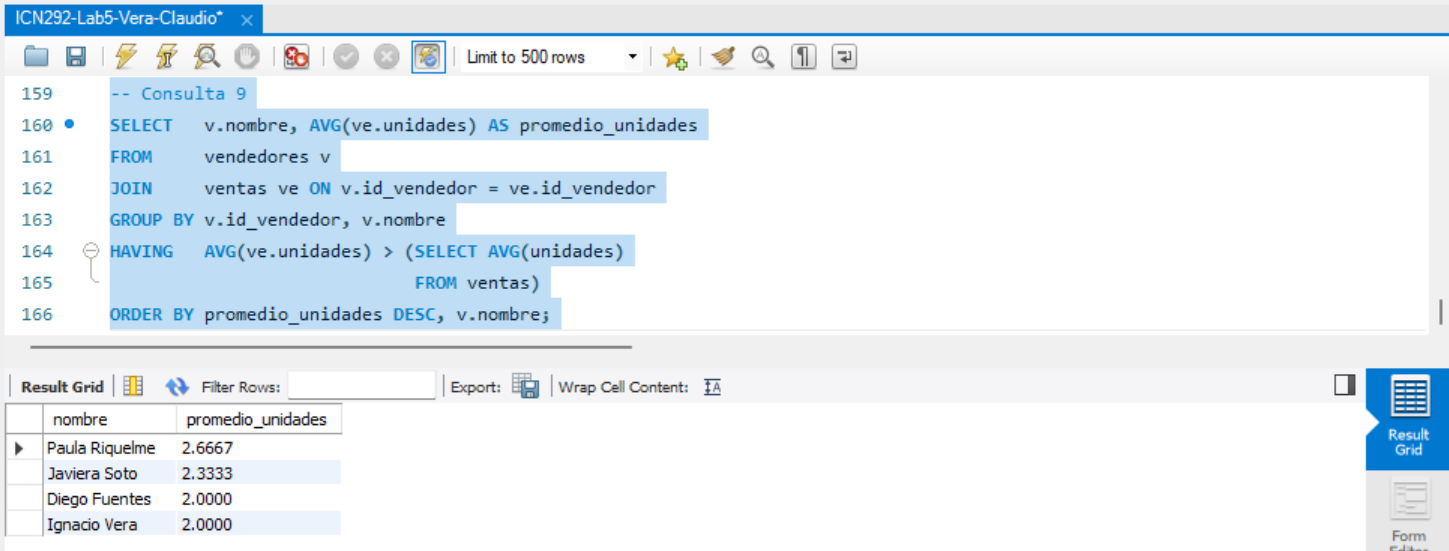
\includegraphics[width=0.72\linewidth]{img/c9.png}
\end{center}
\end{minipage}
\par\vspace{0.6cm}

\noindent\begin{minipage}{\linewidth}
\section*{Consulta 10}

Liste todos los vendedores con el monto total que vendieron, incluidos los que no vendieron nada, de mayor a menor monto. Explique en una línea por qué algunos vendedores no muestran cero y qué tendría que agregar a la consulta para que lo mostraran.

\begin{lstlisting}
SELECT   v.nombre, SUM(ve.unidades * b.precio) AS monto_total
FROM     vendedores v
LEFT JOIN ventas     ve ON v.id_vendedor  = ve.id_vendedor
LEFT JOIN bicicletas b  ON ve.id_bicicleta = b.id_bicicleta
GROUP BY v.id_vendedor, v.nombre
ORDER BY monto_total DESC;
\end{lstlisting}

\begin{center}
    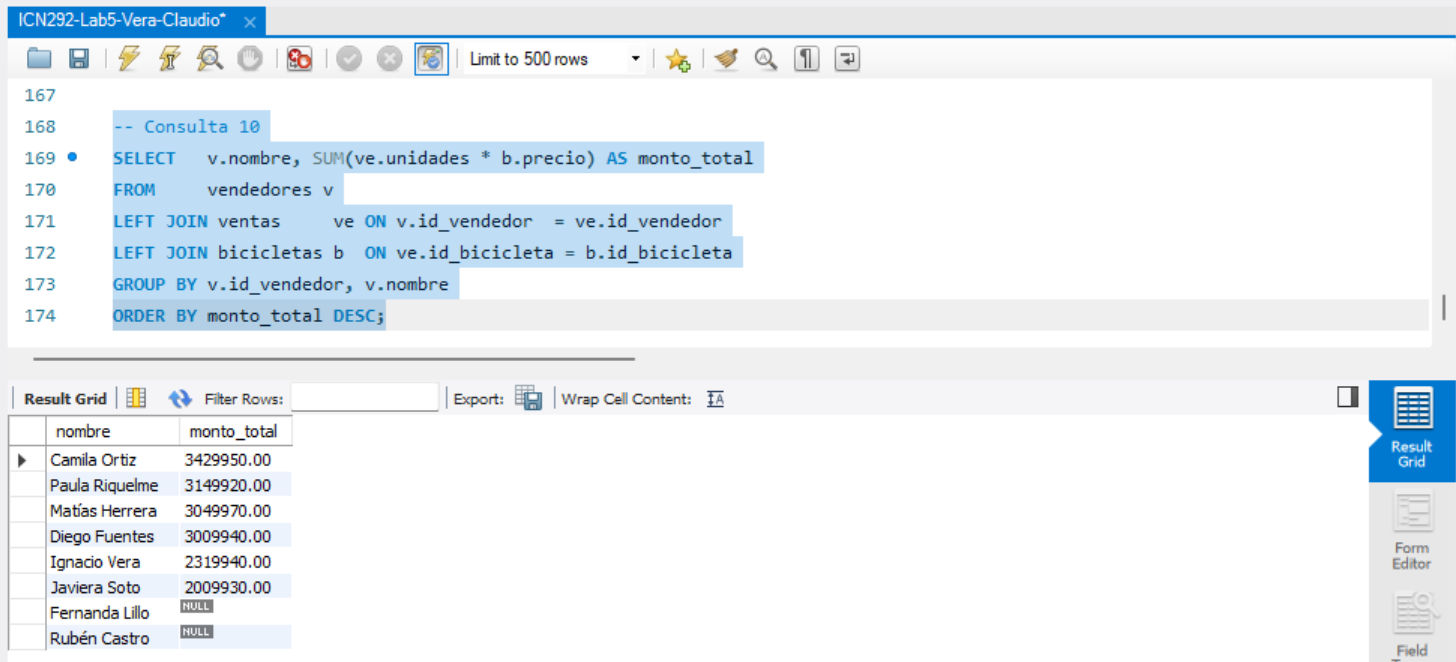
\includegraphics[width=0.72\linewidth]{img/c10.png}
\end{center}

Fernanda Lillo y Rubén Castro salen con NULL porque no tienen ninguna venta, y al no haber nada que sumar el \texttt{SUM} da NULL en vez de 0. Para que salga 0 hay que poner \texttt{IFNULL(SUM(ve.unidades * b.precio), 0)}.
\end{minipage}
\par\vspace{0.6cm}

\end{document}
